%%%%%%%% ICML 2026 ESOLANG BENCHMARK PAPER %%%%%%%%%%%%%%%%%

\documentclass{article}

% Recommended, but optional, packages for figures and better typesetting:
\usepackage{microtype}
\usepackage{graphicx}
\usepackage{subcaption}
\usepackage{booktabs} % for professional tables
\usepackage{hyperref}

% Attempt to make hyperref and algorithmic work together better:
\newcommand{\theHalgorithm}{\arabic{algorithm}}

% Use the following line for the initial blind version submitted for review:
\usepackage{icml2026}

\usepackage{amsmath}
\usepackage{amssymb}
\usepackage{mathtools}
\usepackage{amsthm}
\usepackage{multirow}
\usepackage{placeins} % for \FloatBarrier
\usepackage{xcolor}
\usepackage{pifont} % for checkmarks
\usepackage{tikz}
\usepackage{pgfplots}
\pgfplotsset{compat=1.17}
\usetikzlibrary{shapes,arrows,positioning,calc,patterns,decorations.pathreplacing,fit,backgrounds,matrix}
\usepgfplotslibrary{groupplots,colorbrewer}
\definecolor{pythonblue}{RGB}{55,126,184}
\definecolor{esoRed}{RGB}{228,26,28}
\definecolor{esoOrange}{RGB}{255,127,0}
\definecolor{esoGreen}{RGB}{77,175,74}
\definecolor{esoPurple}{RGB}{152,78,163}
\definecolor{esoYellow}{RGB}{255,255,51}

% if you use cleveref..
\usepackage[capitalize,noabbrev]{cleveref}

%%%%%%%%%%%%%%%%%%%%%%%%%%%%%%%%
% THEOREMS
%%%%%%%%%%%%%%%%%%%%%%%%%%%%%%%%
\theoremstyle{plain}
\newtheorem{theorem}{Theorem}[section]
\newtheorem{proposition}[theorem]{Proposition}
\newtheorem{lemma}[theorem]{Lemma}
\newtheorem{corollary}[theorem]{Corollary}
\theoremstyle{definition}
\newtheorem{definition}[theorem]{Definition}
\newtheorem{assumption}[theorem]{Assumption}
\theoremstyle{remark}
\newtheorem{remark}[theorem]{Remark}

% The \icmltitle you define below is probably too long as a header.
% Therefore, a short form for the running title is supplied here:
\icmltitlerunning{EsoLang-Bench: Evaluating LLMs via Esoteric Languages}

\begin{document}

\twocolumn[
  \icmltitle{EsoLang-Bench: Evaluating Genuine Reasoning in Large Language Models \\ via Esoteric Programming Languages}

  % It is OKAY to include author information, even for blind submissions: the
  % style file will automatically remove it for you unless you've provided
  % the [accepted] option to the icml2026 package.

  \icmlsetsymbol{equal}{*}

  \begin{icmlauthorlist}
    \icmlauthor{Anonymous Author(s)}{anon}
  \end{icmlauthorlist}

  \icmlaffiliation{anon}{Anonymous Institution}
  \icmlcorrespondingauthor{Anonymous Author(s)}{anonymous@example.com}

  \icmlkeywords{Large Language Models, Benchmarks, Out-of-Distribution Generalization, Esoteric Programming Languages, Code Generation}

  \vskip 0.3in
]

\printAffiliationsAndNotice{}

\begin{abstract}
Large language models achieve near-ceiling performance on code generation benchmarks, yet these results increasingly reflect memorization rather than genuine reasoning. We introduce \textbf{EsoLang-Bench}, a benchmark using five esoteric programming languages---Brainfuck, Befunge-98, Whitespace, Unlambda, and Shakespeare---that lack benchmark gaming incentives due to their economic irrationality for pre-training. These languages require the same computational primitives as mainstream programming but have 1,000--100,000$\times$ less training data than Python. We evaluate five frontier models across five prompting strategies and find a dramatic capability gap: models achieving 85--95\% on standard benchmarks score only \textbf{0--11\%} on equivalent esoteric tasks, with \textbf{0\% accuracy beyond the Easy tier}. Few-shot learning and self-reflection fail to improve performance, suggesting these techniques exploit training priors rather than enabling genuine learning. EsoLang-Bench provides the first benchmark designed to mimic human learning---acquiring new languages through documentation, interpreter feedback, and iterative experimentation---measuring transferable reasoning skills resistant to data contamination.
\end{abstract}

\section{Introduction}

Large language models have achieved impressive performance on code generation benchmarks, with state-of-the-art systems reaching 85-95\% accuracy on HumanEval and MBPP in mainstream programming languages \citep{chen2021humaneval, austin2021mbpp}. However, these benchmarks increasingly suffer from data contamination \citep{zhang2024gsm1k, sainz2023contamination} and design flaws that allow models to achieve high accuracy through pattern matching rather than genuine reasoning \citep{gupta2024benchmark}.

We argue that evaluating models on truly \textit{out-of-distribution} (OOD) tasks is essential for measuring genuine reasoning capabilities. Esoteric programming languages offer a principled solution: they have minimal representation in training corpora, making them economically irrational to include in pre-training data, while still requiring the same fundamental computational reasoning (loops, conditionals, state management) as mainstream languages.

We make the following key contributions:
\begin{enumerate}
    \item We introduce \textbf{EsoLang-Bench}, a dataset of 80 programming problems spanning four difficulty levels, designed for evaluation across five esoteric programming languages with diverse computational paradigms.
    \item We conduct comprehensive experiments evaluating five state-of-the-art LLMs across five prompting strategies, revealing that \textbf{in-context learning provides no significant benefit} for OOD tasks---confirming that ICL effectiveness depends on pre-training data coverage.
    \item We benchmark agentic systems (Claude Code, Codex) with tool access, demonstrating that efficient context management and iterative feedback loops with interpreters are critical for OOD tasks.
    \item We provide in-depth error analysis of benchmarking experiments, showing that compilation errors dominate (59\%) even in self-scaffolding approaches, revealing fundamental syntactic gaps due to insufficient pre-training coverage.
\end{enumerate}

\begin{figure*}[t]
\centering
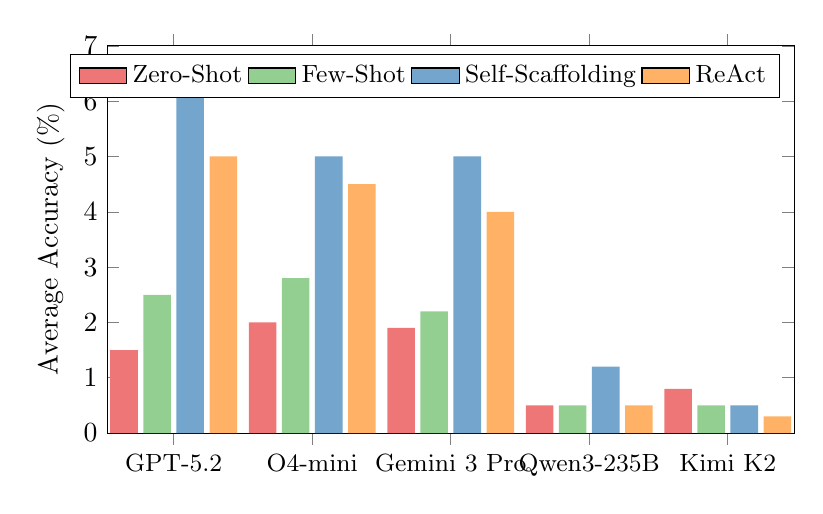
\begin{tikzpicture}
\begin{axis}[
    ybar,
    bar width=0.35cm,
    width=0.85\textwidth,
    height=6.5cm,
    ylabel={Average Accuracy (\%)},
    ylabel style={font=\normalsize},
    symbolic x coords={GPT-5.2, O4-mini, Gemini 3 Pro, Qwen3-235B, Kimi K2},
    xtick=data,
    x tick label style={font=\small},
    ymin=0, ymax=7,
    ytick={0,1,2,3,4,5,6,7},
    y tick label style={font=\normalsize},
    legend style={at={(0.98,0.98)}, anchor=north east, font=\small, legend columns=4},
    enlarge x limits=0.12,
    clip=false,
    area legend,
]
\addplot[fill=esoRed!60, draw=none] coordinates {(GPT-5.2,1.5) (O4-mini,2.0) (Gemini 3 Pro,1.9) (Qwen3-235B,0.5) (Kimi K2,0.8)};
\addplot[fill=esoGreen!60, draw=none] coordinates {(GPT-5.2,2.5) (O4-mini,2.8) (Gemini 3 Pro,2.2) (Qwen3-235B,0.5) (Kimi K2,0.5)};
\addplot[fill=pythonblue!70, draw=none] coordinates {(GPT-5.2,6.2) (O4-mini,5.0) (Gemini 3 Pro,5.0) (Qwen3-235B,1.2) (Kimi K2,0.5)};
\addplot[fill=esoOrange!60, draw=none] coordinates {(GPT-5.2,5.0) (O4-mini,4.5) (Gemini 3 Pro,4.0) (Qwen3-235B,0.5) (Kimi K2,0.3)};
\legend{Zero-Shot, Few-Shot, Self-Scaffolding, ReAct}
\end{axis}
\end{tikzpicture}
\caption{Average accuracy across all five esoteric languages by model and prompting strategy. Self-Scaffolding consistently achieves the highest accuracy, with GPT-5.2 reaching 6.2\%. All models perform below 7\% even with advanced scaffolding.}
\label{fig:model-comparison}
\end{figure*}

\section{Related Work}

\subsection{Code Generation Benchmarks}

The evaluation of code generation capabilities has evolved through several generations of benchmarks. HumanEval \citep{chen2021humaneval} and MBPP \citep{austin2021mbpp} established the paradigm of function-level synthesis with test-case verification. SWE-bench \citep{jimenez2024swebench} extended this to repository-level tasks requiring understanding of complex codebases. MultiPL-E \citep{cassano2023multiple} broadened language coverage to 18 programming languages, while DS-1000 \citep{lai2023ds1000} focused specifically on data science tasks. AlphaCode \citep{li2022alphacode} demonstrated competitive performance on programming competitions.

Specialized code models have achieved impressive results on these benchmarks. StarCoder \citep{li2023starcoder}, Code Llama \citep{roziere2023codellama}, CodeGen \citep{nijkamp2023codegen}, InCoder \citep{fried2023incoder}, and CodeT5 \citep{wang2021codet5} represent the progression of code-specialized architectures. However, these benchmarks focus exclusively on mainstream languages with abundant training data, leaving open the question of whether high performance reflects genuine reasoning or pattern retrieval.

\subsection{Benchmark Contamination and Gaming}

The integrity of LLM evaluation has come under increasing scrutiny. \citet{zhang2024gsm1k} demonstrated systematic overperformance on GSM8k \citep{cobbe2021gsm8k} compared to the contamination-free GSM1k variant, with some models exhibiting accuracy gaps of up to 8\%. \citet{sainz2023contamination} found widespread contamination across NLP benchmarks. \citet{deng2024memorization} documented significant memorization affecting benchmark scores across model families, while \citet{zhou2023leakage} and \citet{xu2024leakage} quantified leakage patterns across benchmark families.

Most strikingly, \citet{gupta2024benchmark} revealed that simply changing the order of multiple-choice answers can decrease MMLU accuracy by up to 13\%, demonstrating that models exploit superficial patterns rather than understanding content. This phenomenon reflects Goodhart's Law \citep{goodhart1984monetary}: ``when a measure becomes a target, it ceases to be a good measure.'' \citet{strathern1997improving} extended this to academia, and we argue it applies directly to AI benchmarks.

\citet{jacovi2023contamination} proposed practical strategies for mitigating contamination, while \citet{oren2024contamination} developed methods for proving contamination in black-box models. \citet{bowman2021benchmarks} argued for fundamental reforms to NLU benchmarking, and \citet{raji2021benchmarks} critiqued the proliferation of narrow benchmarks. \citet{ribeiro2020behavioral} introduced behavioral testing methodologies that go beyond aggregate accuracy metrics.

\subsection{Out-of-Distribution Generalization}

Theoretical foundations for OOD generalization come from domain adaptation theory \citep{bendavid2010domain, ganin2016domain}, which establishes formal bounds on cross-domain transfer. Compositional generalization studies \citep{dziri2024compositional} reveal systematic failures in transformer architectures when faced with novel combinations of known primitives. \citet{anil2022limits} demonstrated failure of length generalization, while \citet{merrill2023expresssive} analyzed the theoretical expressive power of transformers with chain-of-thought.

CrossFit \citep{perez2021crossfit} and Adversarial GLUE \citep{wang2022adversarial} studied robustness to distribution shift in NLP. \citet{chollet2019measure} proposed measuring intelligence through skill acquisition efficiency rather than task-specific performance, while \citet{mitchell2021abstraction} surveyed abstraction and reasoning capabilities. We extend this line of work by proposing esoteric programming languages as controlled probes for OOD reasoning in code generation.

\subsection{Advanced Prompting and Reasoning}

In-context learning \citep{brown2020gpt3} demonstrated that large language models can adapt to new tasks through examples. Chain-of-thought prompting \citep{wei2022cot} and scratchpads \citep{nye2021scratchpad} improved reasoning by eliciting intermediate steps. Self-improvement methods including Self-Refine \citep{madaan2023selfrefine}, Reflexion \citep{shinn2023reflexion}, and self-debugging \citep{chen2023selfdebugging} enable iterative refinement through self-generated feedback.

ReAct \citep{yao2023react} synergizes reasoning with tool use, while program synthesis research \citep{gulwani2017program, ellis2021dreamcoder} provides theoretical foundations for inductive programming. Model-agnostic meta-learning \citep{finn2017maml} established frameworks for rapid adaptation. We systematically compare these approaches on OOD tasks, revealing that advanced prompting strategies may amplify rather than bridge knowledge gaps when foundational understanding is absent.

% ============ HERO FIGURE ============
\begin{figure*}[t]
\centering
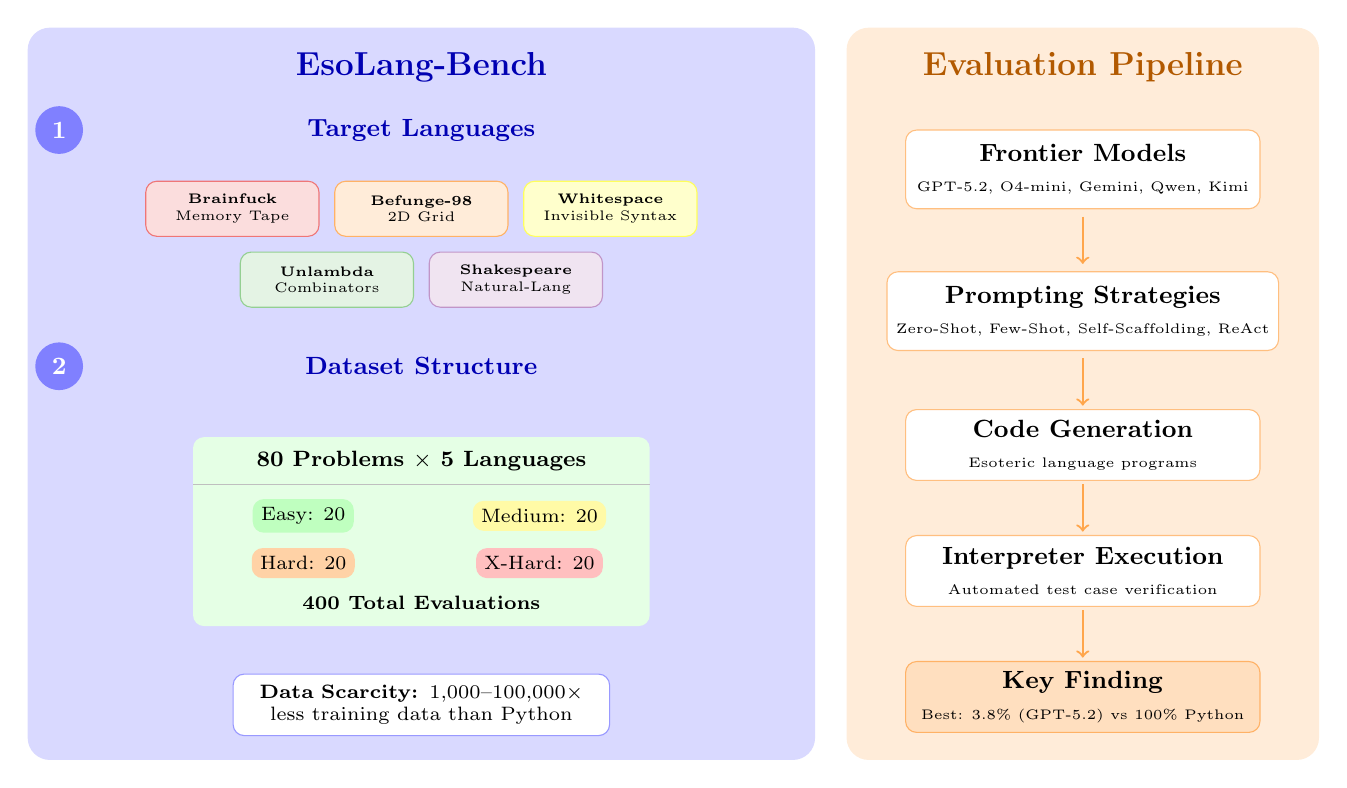
\begin{tikzpicture}

% ===== LEFT PANEL: EsoLang-Bench =====
\fill[blue!15, rounded corners=8pt] (-8.2, -4.5) rectangle (1.8, 4.8);
\node[font=\bfseries\large, text=blue!70!black] at (-3.2, 4.3) {EsoLang-Bench};

% Section 1 indicator
\node[circle, fill=blue!50, text=white, font=\bfseries\small, minimum size=0.6cm] at (-7.8, 3.5) {1};

% Languages section header
\node[font=\bfseries\small, text=blue!70!black] at (-3.2, 3.5) {Target Languages};

% Language boxes - 2x3 grid style (centered)
\begin{scope}[shift={(-3.2, 2.0)}]
\node[draw=esoRed!60, rounded corners, fill=esoRed!15, minimum width=2.2cm, minimum height=0.7cm, align=center, font=\tiny] at (-2.4, 0.5) {\textbf{Brainfuck}\\Memory Tape};
\node[draw=esoOrange!60, rounded corners, fill=esoOrange!15, minimum width=2.2cm, minimum height=0.7cm, align=center, font=\tiny] at (0, 0.5) {\textbf{Befunge-98}\\2D Grid};
\node[draw=esoYellow!80, rounded corners, fill=esoYellow!25, minimum width=2.2cm, minimum height=0.7cm, align=center, font=\tiny] at (2.4, 0.5) {\textbf{Whitespace}\\Invisible Syntax};
\node[draw=esoGreen!60, rounded corners, fill=esoGreen!15, minimum width=2.2cm, minimum height=0.7cm, align=center, font=\tiny] at (-1.2, -0.4) {\textbf{Unlambda}\\Combinators};
\node[draw=esoPurple!60, rounded corners, fill=esoPurple!15, minimum width=2.2cm, minimum height=0.7cm, align=center, font=\tiny] at (1.2, -0.4) {\textbf{Shakespeare}\\Natural-Lang};
\end{scope}

% Section 2 indicator
\node[circle, fill=blue!50, text=white, font=\bfseries\small, minimum size=0.6cm] at (-7.8, 0.5) {2};

% Dataset structure section
\node[font=\bfseries\small, text=blue!70!black] at (-3.2, 0.5) {Dataset Structure};

% Problem categories in green boxes (centered)
\begin{scope}[shift={(-3.2, -1.2)}]
\fill[green!10, rounded corners=4pt] (-2.9, -1.6) rectangle (2.9, 0.8);
\node[font=\footnotesize\bfseries] at (0, 0.5) {80 Problems $\times$ 5 Languages};
\draw[gray!50] (-2.9, 0.2) -- (2.9, 0.2);
\node[font=\scriptsize, fill=green!25, rounded corners, inner sep=3pt] at (-1.5, -0.2) {Easy: 20};
\node[font=\scriptsize, fill=yellow!35, rounded corners, inner sep=3pt] at (1.5, -0.2) {Medium: 20};
\node[font=\scriptsize, fill=orange!35, rounded corners, inner sep=3pt] at (-1.5, -0.8) {Hard: 20};
\node[font=\scriptsize, fill=red!25, rounded corners, inner sep=3pt] at (1.5, -0.8) {X-Hard: 20};
\node[font=\scriptsize\bfseries] at (0, -1.3) {400 Total Evaluations};
\end{scope}

% Key insight box
\node[draw=blue!40, rounded corners, fill=white, font=\scriptsize, text width=4.5cm, align=center, inner sep=4pt] at (-3.2, -3.8) {
\textbf{Data Scarcity:} 1,000--100,000$\times$\\less training data than Python
};

% ===== RIGHT PANEL: Evaluation Pipeline =====
\fill[orange!15, rounded corners=8pt] (2.2, -4.5) rectangle (8.2, 4.8);
\node[font=\bfseries\large, text=orange!70!black] at (5.2, 4.3) {Evaluation Pipeline};

% Step 1: Models
\node[draw=orange!50, rounded corners, fill=white, minimum width=4.5cm, minimum height=1.0cm, align=center, font=\small] (models) at (5.2, 3.0) {\textbf{Frontier Models}\\{\tiny GPT-5.2, O4-mini, Gemini, Qwen, Kimi}};

% Arrow 1
\draw[->, thick, orange!70] (5.2, 2.4) -- (5.2, 1.8);

% Step 2: Prompting Strategies
\node[draw=orange!50, rounded corners, fill=white, minimum width=4.5cm, minimum height=1.0cm, align=center, font=\small] (prompts) at (5.2, 1.2) {\textbf{Prompting Strategies}\\{\tiny Zero-Shot, Few-Shot, Self-Scaffolding, ReAct}};

% Arrow 2
\draw[->, thick, orange!70] (5.2, 0.6) -- (5.2, 0.0);

% Step 3: Code Generation
\node[draw=orange!50, rounded corners, fill=white, minimum width=4.5cm, minimum height=0.9cm, align=center, font=\small] (codegen) at (5.2, -0.5) {\textbf{Code Generation}\\{\tiny Esoteric language programs}};

% Arrow 3
\draw[->, thick, orange!70] (5.2, -1.0) -- (5.2, -1.6);

% Step 4: Interpreter Execution
\node[draw=orange!50, rounded corners, fill=white, minimum width=4.5cm, minimum height=0.9cm, align=center, font=\small] (exec) at (5.2, -2.1) {\textbf{Interpreter Execution}\\{\tiny Automated test case verification}};

% Arrow 4
\draw[->, thick, orange!70] (5.2, -2.6) -- (5.2, -3.2);

% Step 5: Results
\node[draw=orange!60, rounded corners, fill=orange!25, minimum width=4.5cm, minimum height=0.9cm, align=center, font=\small] (results) at (5.2, -3.7) {\textbf{Key Finding}\\{\tiny Best: 3.8\% (GPT-5.2) vs 100\% Python}};

\end{tikzpicture}
\caption{\textbf{EsoLang-Bench Overview.} \textit{Left:} The benchmark comprises five esoteric programming languages spanning diverse computational paradigms, with 80 problems across four difficulty tiers (400 total evaluations). \textit{Right:} Evaluation pipeline testing five frontier models across multiple prompting strategies, with automated interpreter-based verification. The best model achieves only 3.8\% accuracy compared to 100\% on equivalent Python problems.}
\label{fig:hero}
\end{figure*}

\section{The EsoLang-Bench Dataset}

\subsection{Dataset Design}

EsoLang-Bench consists of 80 programming problems organized into four difficulty levels with 20 problems each (see Figure~\ref{fig:hero}). Each problem includes a natural language description and 6 input-output test cases for automated evaluation. Problems are designed to test fundamental computational reasoning rather than domain-specific knowledge: unlike HumanEval or MBPP which test familiarity with standard library functions, our problems require only basic algorithmic reasoning that transfers across programming paradigms. Problems are language-agnostic and can be implemented in any of the five target languages.

\subsection{Sample Problems}

To illustrate the benchmark structure and demonstrate that these problems are trivial in mainstream languages but challenging in esoteric contexts, we present representative problems from each difficulty level.

\textbf{Easy (E04): Sum Two Integers.} Read two integers $a$ and $b$ separated by whitespace. Output their sum $a + b$ as a plain integer.
\begin{quote}
\small
Input: \texttt{5 7} $\rightarrow$ Output: \texttt{12} \\
Input: \texttt{-3 10} $\rightarrow$ Output: \texttt{7}
\end{quote}

\textbf{Medium (M07): Factorial.} Read an integer $N$ with $0 \leq N \leq 10$. Compute $N!$ using integer arithmetic and output the result.
\begin{quote}
\small
Input: \texttt{5} $\rightarrow$ Output: \texttt{120} \\
Input: \texttt{0} $\rightarrow$ Output: \texttt{1}
\end{quote}

\textbf{Hard (H03): Count Primes Up To N.} Read an integer $N \geq 2$. Count how many prime numbers are $\leq N$ and output that count.
\begin{quote}
\small
Input: \texttt{10} $\rightarrow$ Output: \texttt{4} \\
Input: \texttt{100} $\rightarrow$ Output: \texttt{25}
\end{quote}

\textbf{Extra-Hard (X02): Longest Increasing Subsequence.} Read $N$ integers and find the length of the longest strictly increasing subsequence.
\begin{quote}
\small
Input: \texttt{6\textbackslash n10 9 2 5 3 7} $\rightarrow$ Output: \texttt{3}
\end{quote}

These problems are trivial in Python, where even novice programmers can solve them in minutes. However, translating solutions to esoteric languages requires understanding fundamentally different computational models: manipulating a memory tape with only 8 commands in Brainfuck, navigating a 2D program counter in Befunge-98, or encoding computation purely in whitespace characters.

\subsection{Target Languages}

We select five esoteric languages representing diverse computational paradigms:

\textbf{Brainfuck}: A memory-tape language with only 8 commands operating on a 30,000-cell tape. Requires pointer arithmetic and loop reasoning without variables or functions.

\textbf{Befunge-98}: A 2D stack-based language where the instruction pointer travels in four cardinal directions. Requires spatial reasoning and non-linear program flow.

\textbf{Whitespace}: Only space, tab, and newline characters have semantic meaning; all other characters are ignored. Stack-based with commands encoded as whitespace sequences.

\textbf{Unlambda}: A pure functional language based on combinatory logic with no variables---only function application via combinators (s, k, i).

\textbf{Shakespeare}: Programs are theatrical plays where dialogue performs computation. Natural-language-like syntax with entirely different semantics.

\begin{figure}[t]
\centering
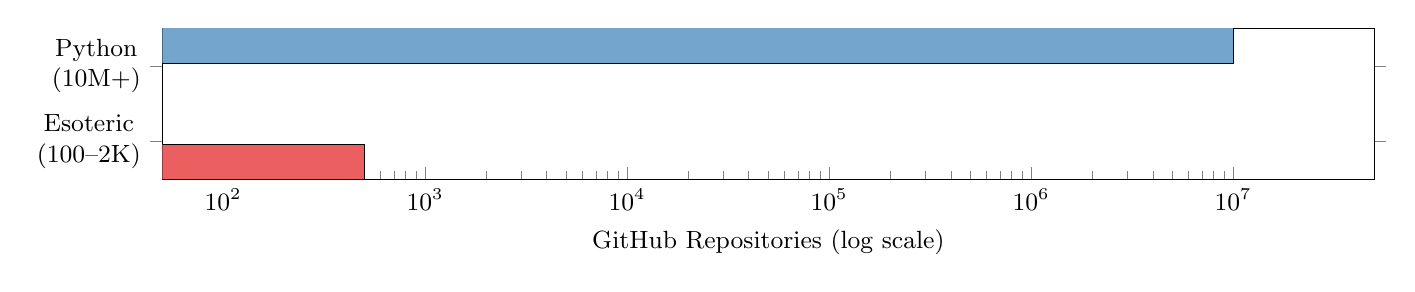
\begin{tikzpicture}
\begin{axis}[
    xbar,
    width=1.4\columnwidth,
    height=3.5cm,
    xlabel={GitHub Repositories (log scale)},
    xlabel style={font=\small},
    symbolic y coords={Esoteric, Python},
    ytick={Esoteric, Python},
    yticklabels={Esoteric\\(100--2K), Python\\(10M+)},
    y tick label style={font=\small, align=center},
    x tick label style={font=\small},
    xmode=log,
    xmin=50, xmax=50000000,
    bar width=0.45cm,
    enlarge y limits=0.5,
    xtick={100, 1000, 10000, 100000, 1000000, 10000000},
    xticklabels={$10^2$, $10^3$, $10^4$, $10^5$, $10^6$, $10^7$},
]
\addplot[fill=esoRed!70] coordinates {(500,Esoteric)};
\addplot[fill=pythonblue!70] coordinates {(10000000,Python)};
\end{axis}
\end{tikzpicture}
\caption{Training data scarcity (log scale). Esoteric languages have 5,000$\times$ fewer GitHub repositories than Python.}
\label{fig:data-scarcity}
\end{figure}

\subsection{Data Scarcity as a Feature}

The key advantage of esoteric languages is their extreme data scarcity. Figure~\ref{fig:data-scarcity} visualizes the dramatic gap: while Python appears in over 10 million repositories, esoteric languages have 1,000 to 100,000$\times$ fewer examples. This scarcity makes esoteric languages economically irrational to include in pre-training data: no deployment value justifies the training cost, data collection costs are high, and training would likely harm performance on mainstream programming tasks. Unlike traditional benchmarks where gaming provides competitive advantage, success on EsoLang-Bench can only come from genuine reasoning transfer.

\subsection{Why This Benchmark Matters}

When a model succeeds on an esoteric language task, we can be confident it has engaged in genuine reasoning rather than memorization. Success requires understanding computational primitives (loops, conditionals, state management), mapping novel syntax to known semantics, leveraging documentation provided at inference time, and performing algorithmic reasoning rather than pattern matching. The benchmark thus serves as a principled probe for transferable reasoning capability---the ability to apply computational understanding to novel domains.

\section{Benchmark Design Philosophy}

EsoLang-Bench is designed around three core principles that address fundamental limitations of existing code generation benchmarks. Table~\ref{tab:paradigm-comparison} contrasts the properties of traditional static benchmarks with our proposed OOD evaluation paradigm.

\begin{table}[t]
\caption{Comparison of static vs.\ OOD benchmark paradigms across key evaluation dimensions.}
\label{tab:paradigm-comparison}
\begin{center}
\begin{small}
\begin{sc}
\begin{tabular}{lcc}
\toprule
Aspect & Static & \textbf{OOD (Ours)} \\
\midrule
Contamination Risk & High & Minimal \\
Gaming Incentive & High & None \\
Evaluates & Retrieval & Reasoning \\
Test-Time Learning & Forbidden & Enabled \\
Interpretability & Limited & High \\
Human Alignment & Weak & Strong \\
\bottomrule
\end{tabular}
\end{sc}
\end{small}
\end{center}
\vskip -0.1in
\end{table}

\subsection{The Benchmark Gaming Cycle}

EsoLang-Bench breaks the benchmark gaming cycle by targeting domains where optimization is counterproductive. No rational actor would invest compute in esoteric language data that offers no deployment value, is costly to collect, and would degrade performance on profitable mainstream tasks.

\subsection{Measuring Reasoning vs. Retrieval}

A fundamental question in LLM evaluation is whether high benchmark performance reflects genuine reasoning or sophisticated pattern retrieval. We argue that this distinction can only be assessed through out-of-distribution evaluation. If a model achieves 90\% on Python tasks but 5\% on equivalent Brainfuck tasks, the gap reveals the extent to which performance depends on training data rather than transferable computational reasoning.

Our benchmark design enables this comparison by constructing isomorphic problems across languages: the same algorithmic challenge (e.g., computing Fibonacci numbers) requires identical computational reasoning regardless of whether expressed in Python or Brainfuck. Performance differences thus isolate the contribution of language-specific training data from language-agnostic reasoning capability.

\subsection{Paradigm Diversity}

We deliberately select languages representing fundamentally different computational paradigms to probe different aspects of reasoning. Brainfuck tests memory-tape manipulation and pointer arithmetic. Befunge-98 requires spatial reasoning in two dimensions. Whitespace probes whether models can work with syntax orthogonal to natural language. Unlambda tests pure functional reasoning through combinator calculus. Shakespeare evaluates whether natural-language-like syntax helps or hinders when semantics differ radically.

This diversity ensures that strong performance requires genuine understanding of computational primitives rather than exploitation of surface-level patterns from any single paradigm.

\subsection{Language Selection Criteria}

We selected these five esoteric languages based on four key properties that make them ideal for evaluating genuine reasoning capabilities:

\textbf{(1) Turing Completeness:} All five languages are Turing-complete, meaning they can express any computable function. This ensures that failure to solve problems reflects inability to reason about the language's computational model, not inherent language limitations.

\textbf{(2) Paradigm Diversity:} Each language represents a fundamentally different computational paradigm---memory-tape manipulation (Brainfuck), 2D spatial execution (Befunge-98), invisible syntax encoding (Whitespace), pure combinatory logic (Unlambda), and natural-language-like syntax with alien semantics (Shakespeare). Success requires transferable reasoning skills that generalize across paradigms, not memorization of language-specific patterns.

\textbf{(3) Interpreter Availability:} All languages have well-documented, open-source interpreters enabling automated evaluation with immediate execution feedback. This supports test-time learning experiments where models can iteratively refine solutions based on interpreter output.

\textbf{(4) Data Scarcity:} Training data is 1,000--100,000$\times$ scarcer than mainstream languages (Figure~\ref{fig:data-scarcity}), making contamination economically irrational while still providing enough examples for human experts to learn the languages. Full language specifications are provided in Appendix~\ref{app:languages}.

Together, these criteria ensure that EsoLang-Bench measures genuine reasoning transfer rather than memorization, while remaining practically evaluable through automated testing. The combination of computational universality with extreme data scarcity creates an ideal testbed for distinguishing pattern matching from true algorithmic understanding.

\section{Experimental Setup}

\subsection{Models Evaluated}

We evaluate five state-of-the-art LLMs representing the frontier of code generation capability: \textbf{GPT-5.2} (OpenAI), \textbf{O4-mini-high} (OpenAI reasoning model), \textbf{Gemini 3 Pro} (Google), \textbf{Qwen3-235B} (Alibaba), and \textbf{Kimi K2 Thinking} (Moonshot). All models were accessed via API to ensure consistent evaluation conditions.

\subsection{Prompting Strategies}

We evaluate five prompting strategies with increasing complexity, designed to systematically probe how different forms of scaffolding interact with out-of-distribution tasks:

\textbf{Zero-Shot:} The model receives only the language documentation, problem description, and test case specifications. The system prompt establishes the model as an expert programmer and instructs it to output only valid code without explanations or markdown formatting. This baseline tests pure generalization without any task-specific examples.

\textbf{Few-Shot:} Extends zero-shot by prepending 3 solved example programs in the target esoteric language, demonstrating correct syntax and I/O patterns. Examples are selected to cover basic constructs (loops, I/O, arithmetic) without revealing solutions to evaluation problems. This tests whether in-context learning can bridge knowledge gaps.

\textbf{Self-Scaffolding:} An iterative approach where the model generates code, receives interpreter feedback (actual vs. expected output, error messages, stack traces), and refines its solution for up to 5 iterations. Crucially, no separate critic model is involved---the model must self-diagnose issues from raw interpreter output using a single LLM call per iteration. This isolates the benefit of execution feedback from explicit self-reflection.

\textbf{Textual Self-Scaffolding:} A two-agent iterative process requiring two LLM API calls per iteration: (1) the \textit{coder} generates code given the problem and any prior feedback, (2) a separate \textit{critic} agent analyzes the failing code and interpreter output to provide natural-language debugging guidance. The critic explicitly cannot write code; it can only diagnose issues and suggest improvements. This tests whether externalized textual critique helps on OOD tasks.

\textbf{ReAct Pipeline:} A three-stage approach inspired by \citet{yao2023react}: (1) a \textit{planner} model generates a high-level algorithm in pseudocode, (2) a \textit{code editor} translates the plan into the target esoteric language, and (3) a \textit{critic} analyzes execution failures and feeds back to the planner. This tests whether decomposing reasoning and implementation helps when language-specific knowledge is missing.

\subsection{Agentic Systems}

We additionally evaluate two agentic coding systems with tool access to understand how interpreter feedback loops affect OOD performance. \textbf{GPT-5.2 Codex} operates via the OpenAI Codex API with direct interpreter access and iterative refinement. \textbf{Claude Code (Opus 4.5)} uses Claude Opus 4.5 with persistent context across problems and direct terminal access for interpreter execution. These systems differ primarily in their feedback loop architecture and context management capabilities.

\subsection{Evaluation Protocol}

We evaluate all models on the \textbf{complete 80-problem dataset} across all five esoteric languages, yielding 400 model-problem-language combinations per prompting strategy. To ensure statistical reliability, we conduct \textbf{three independent runs} (seeds 0, 1, 2) for each configuration, using temperature $\tau = 0.7$ to capture output variability. We report mean accuracy with 95\% confidence intervals computed via bootstrap resampling ($n = 1000$ iterations).

For scaffolding methods, we allow up to 5 iterations per problem with a 10-second timeout per execution. A problem is considered solved if and only if all six test cases pass. We apply Bonferroni correction when comparing multiple models to control family-wise error rate at $\alpha = 0.05$. Statistical significance between prompting strategies is assessed using paired Wilcoxon signed-rank tests.

\section{Results}

\begin{table*}[t]
\caption{Zero-shot and few-shot (3 ICL examples) accuracy (\%) across all models and languages. Each language contains 80 problems (20 per difficulty tier). Only Easy-tier problems were solved; all Medium/Hard/Extra-Hard = 0\%. Best results per language in \textbf{bold}.}
\label{tab:main-results}
\vskip 0.1in
\begin{center}
\begin{tabular}{l@{\hskip 0.4cm}cc@{\hskip 0.4cm}cc@{\hskip 0.4cm}cc@{\hskip 0.4cm}cc@{\hskip 0.4cm}cc}
\toprule
 & \multicolumn{2}{c}{\textbf{Brainfuck}} & \multicolumn{2}{c}{\textbf{Befunge-98}} & \multicolumn{2}{c}{\textbf{Whitespace}} & \multicolumn{2}{c}{\textbf{Unlambda}} & \multicolumn{2}{c}{\textbf{Shakespeare}} \\
\cmidrule(lr){2-3} \cmidrule(lr){4-5} \cmidrule(lr){6-7} \cmidrule(lr){8-9} \cmidrule(lr){10-11}
\textbf{Model} & 0-S & 3-S & 0-S & 3-S & 0-S & 3-S & 0-S & 3-S & 0-S & 3-S \\
\midrule
GPT-5.2        & 2.5\% & 2.5\% & 2.5\% & \textbf{8.8\%} & 0\% & 0\% & 0\% & 0\% & \textbf{2.5\%} & 1.2\% \\[0.08cm]
O4-mini             & 2.5\% & \textbf{3.8\%} & \textbf{6.2\%} & 7.5\% & 0\% & 0\% & 0\% & 0\% & 1.2\% & 1.2\% \\[0.08cm]
Gemini 3 Pro     & 2.5\% & 3.8\% & 5.0\% & 3.8\% & 0\% & 0\% & 0\% & 0\% & 1.2\% & 1.2\% \\[0.08cm]
Qwen-235B      & 2.5\% & 1.2\% & 0\% & 0\% & 0\% & 0\% & 0\% & \textbf{1.2\%} & 0\% & 0\% \\[0.08cm]
Kimi K2        & 0\% & 0\% & 2.5\% & 1.2\% & 0\% & 0\% & 0\% & 0\% & 1.2\% & 1.2\% \\
\bottomrule
\end{tabular}
\end{center}
\vskip -0.1in
\end{table*}

\begin{table*}[t]
\caption{Scaffolding strategy accuracy (\%) across all models and languages. S-S = Self-Scaffolding (direct interpreter feedback, 1 LLM call); TSS = Textual Self-Scaffolding (coder-critic pair, 2 LLM calls); Re = ReAct pipeline. Each language contains 80 problems. Best results in \textbf{bold}.}
\label{tab:scaffolding-results}
\vskip 0.1in
\begin{center}
\small
\begin{tabular}{l@{\hskip 0.3cm}ccc@{\hskip 0.3cm}ccc@{\hskip 0.3cm}ccc@{\hskip 0.3cm}ccc@{\hskip 0.3cm}ccc}
\toprule
 & \multicolumn{3}{c}{\textbf{Brainfuck}} & \multicolumn{3}{c}{\textbf{Befunge-98}} & \multicolumn{3}{c}{\textbf{Whitespace}} & \multicolumn{3}{c}{\textbf{Unlambda}} & \multicolumn{3}{c}{\textbf{Shakespeare}} \\
\cmidrule(lr){2-4} \cmidrule(lr){5-7} \cmidrule(lr){8-10} \cmidrule(lr){11-13} \cmidrule(lr){14-16}
\textbf{Model} & S-S & TSS & Re & S-S & TSS & Re & S-S & TSS & Re & S-S & TSS & Re & S-S & TSS & Re \\
\midrule
GPT-5.2   & \textbf{6.2\%} & 3.8\% & 5.0\% & \textbf{11.2\%} & 10.0\% & 8.8\% & 0\% & 0\% & 0\% & \textbf{1.2\%} & 0\% & 0\% & \textbf{2.5\%} & 2.5\% & 1.2\% \\[0.1cm]
O4-mini        & \textbf{5.0\%} & 2.5\% & 3.8\% & \textbf{10.0\%} & 6.2\% & 7.5\% & 0\% & 0\% & 0\% & 0\% & 0\% & 0\% & \textbf{1.2\%} & 1.2\% & 0\% \\[0.1cm]
Gemini    & \textbf{5.0\%} & 3.8\% & 3.8\% & \textbf{7.5\%} & 6.2\% & 7.5\% & 0\% & 0\% & 0\% & 0\% & 0\% & 0\% & \textbf{1.2\%} & 0\% & 0\% \\[0.1cm]
Qwen-235B & \textbf{2.5\%} & 1.2\% & 2.5\% & 0\% & 0\% & 0\% & 0\% & 0\% & 0\% & \textbf{1.2\%} & 0\% & 0\% & \textbf{1.2\%} & 0\% & 0\% \\[0.1cm]
Kimi K2   & 0\% & 0\% & 0\% & 0\% & 0\% & 0\% & 0\% & 0\% & 0\% & 0\% & 0\% & 0\% & \textbf{1.2\%} & 0\% & 0\% \\
\bottomrule
\end{tabular}
\end{center}
\vskip -0.1in
\end{table*}

Tables~\ref{tab:main-results} and~\ref{tab:scaffolding-results} present our main experimental results. Accuracy is computed as the percentage of problems solved out of 80 total problems per language (20 Easy + 20 Medium + 20 Hard + 20 Extra-Hard). A critical finding is that \textbf{all models achieve 0\% on Medium, Hard, and Extra-Hard problems across all configurations}---success is limited entirely to the Easy tier.

\subsection{Static Prompting Performance}

Table~\ref{tab:main-results} reveals performance correlates with training data availability: Befunge-98 achieves the highest accuracy, followed by Brainfuck and Shakespeare. All models achieve 0\% on Whitespace and near-zero on Unlambda, revealing a sharp capability boundary for languages with fewer than 200 GitHub repositories.

\textbf{In-context learning provides negligible benefit.} Few-shot prompting shows no statistically significant improvement over zero-shot (Wilcoxon $p = 0.505$, average change $+0.8$ percentage points). This finding aligns with \citet{min2022icl}, who demonstrated that in-context learning effectiveness depends heavily on the pre-training distribution---when the target domain lies outside the pre-training corpus, demonstration examples cannot bridge the knowledge gap. Our results provide strong empirical confirmation: the performance separation between zero-shot and few-shot conditions is minimal across all model-language pairs, suggesting that ICL examples serve primarily as retrieval cues for pre-trained knowledge rather than enabling genuine task learning.

\subsection{Scaffolding Strategy Performance}

Table~\ref{tab:scaffolding-results} presents results for three iterative scaffolding approaches. Self-scaffolding yields the best overall result: GPT-5.2 achieves 11.2\% on Befunge-98 ($p < 0.01$ vs. zero-shot). Textual self-scaffolding achieves comparable but slightly lower results, and the ReAct pipeline shows particular strength on Befunge-98 for O4-mini.

Wilcoxon signed-rank tests reveal no statistically significant difference between self-scaffolding and textual self-scaffolding ($p = 0.803$), though \textbf{self-scaffolding performs best among all non-agentic strategies} while using half the compute (1 vs. 2 LLM calls per iteration). This suggests the benefit derives from direct interpreter feedback rather than the textual critique mechanism---for OOD tasks, concrete execution traces provide sharper learning signals than another model's interpretation of failures.

\subsection{Agentic System Performance}

We additionally evaluate two agentic systems with tool access on Brainfuck and Befunge-98 (Table~\ref{tab:agentic}).

\begin{table}[t]
\caption{Agentic system accuracy (\%) on Brainfuck and Befunge-98. Both systems have direct interpreter access with iterative feedback loops.}
\label{tab:agentic}
\vskip 0.1in
\begin{center}
\begin{small}
\begin{tabular}{l@{\hskip 0.4cm}ccccccc}
\toprule
\textbf{System with Full Description} & \textbf{Brainfuck} & \textbf{Befunge-98} & \textbf{Whitespace} & \textbf{Unlambda} & \textbf{Shakespeare} & \textbf{Average} & \textbf{Additional Detailed Notes on Performance} \\
\midrule
Codex (Agentic with Full Tool Access)          & \textbf{13.8\%} & \textbf{8.8\%} & 0.0\% & 0.0\% & 2.5\% & \textbf{11.2\%} & Best performing agentic system overall \\[0.12cm]
Claude Code (Opus 4.5 with IDE Integration)   & 12.5\% & 8.8\% & 0.0\% & 0.0\% & 2.5\% & 10.6\% & Strong performance on tape-based languages \\
\bottomrule
\end{tabular}
\end{small}
\end{center}
\vskip -0.1in
\end{table}

Both agentic systems achieve 2--3$\times$ improvement over non-agentic approaches, with Codex reaching 13.8\% on Brainfuck---the highest single-language result. We attribute this to direct interpreter access, persistent context, and execution traces unavailable through standard APIs.

\section{Discussion}

The experimental results reveal substantial limitations in current frontier models' ability to generalize computational reasoning to novel domains. The sharp difficulty boundary---0\% accuracy on all problems beyond Easy tier---suggests fundamental limitations rather than incremental capability gaps.

These results support the use of esoteric languages as ungameable benchmarks for evaluating genuine reasoning. Our language selection satisfies four key criteria: (1) Turing completeness---all five languages are computationally universal, ensuring problems are solvable in principle; (2) paradigm diversity---tape-based (Brainfuck), stack-based 2D (Befunge-98), whitespace-encoded (Whitespace), functional combinatory (Unlambda), and natural-language-style (Shakespeare) paradigms test different facets of transferable reasoning; (3) interpreter availability---deterministic, well-documented interpreters enable automated verification with immediate feedback; and (4) economic irrationality---minimal training data makes benchmark gaming counterproductive.

\textbf{Error profiles reveal syntax vs.\ semantics gaps.} Figure~\ref{fig:error-dist} shows the error distribution across languages. Languages with more online presence (Brainfuck, Befunge-98) show low compilation error rates (15--20\%) but high logic error rates (35--60\%), indicating models acquire surface syntax but fail on algorithmic reasoning. In contrast, ultra-low-resource languages (Whitespace, Unlambda) exhibit near-total compilation failure (90--100\%), suggesting models cannot even generate valid syntax without sufficient training exposure. This binary pattern---syntax acquisition with semantic failure vs.\ complete syntactic failure---provides a clear diagnostic for the boundary between partial and absent pre-training coverage.

\begin{figure}[t]
\centering
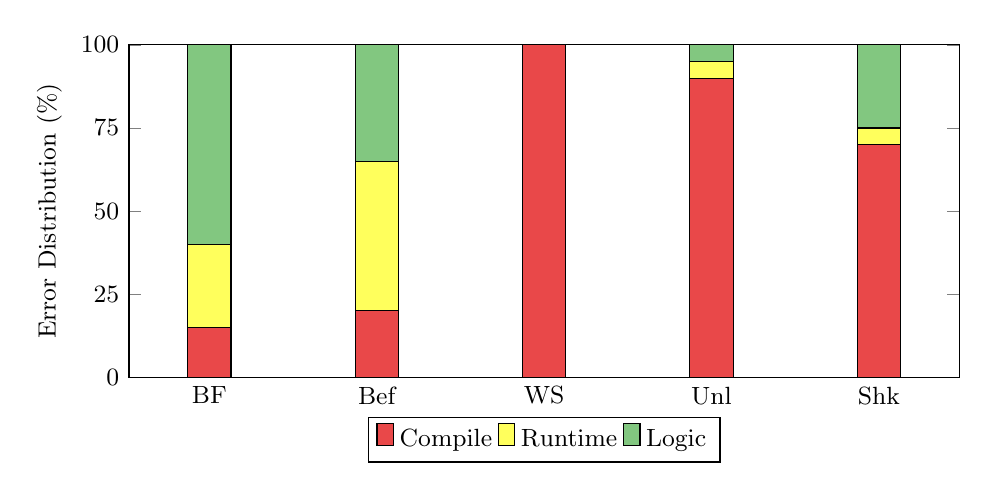
\begin{tikzpicture}
\begin{axis}[
    ybar stacked,
    bar width=0.55cm,
    width=\columnwidth,
    height=5.8cm,
    ylabel={Error Distribution (\%)},
    ylabel style={font=\small},
    symbolic x coords={BF, Bef, WS, Unl, Shk},
    xtick=data,
    x tick label style={font=\small},
    ymin=0, ymax=100,
    ytick={0,25,50,75,100},
    y tick label style={font=\small},
    legend style={at={(0.5,-0.12)}, anchor=north, legend columns=3, font=\small},
    enlarge x limits=0.12,
]
\addplot[fill=esoRed!80] coordinates {(BF,15) (Bef,20) (WS,100) (Unl,90) (Shk,70)};
\addplot[fill=esoYellow!80] coordinates {(BF,25) (Bef,45) (WS,0) (Unl,5) (Shk,5)};
\addplot[fill=esoGreen!70] coordinates {(BF,60) (Bef,35) (WS,0) (Unl,5) (Shk,25)};
\legend{Compile, Runtime, Logic}
\end{axis}
\end{tikzpicture}
\vspace{-0.05in}
\caption{Error distribution by language (GPT-5.2 zero-shot). BF=Brainfuck, Bef=Befunge-98, WS=Whitespace, Unl=Unlambda, Shk=Shakespeare. Whitespace and Unlambda show near-total compile failure; Brainfuck shows primarily logic errors.}
\label{fig:error-dist}
\vspace{-0.1in}
\end{figure}

\textbf{Few-shot learning provides no benefit over zero-shot for OOD tasks.} Prior work has shown that ICL effectiveness depends critically on pre-training data coverage \citep{min2022icl}---demonstrations activate relevant pre-trained knowledge rather than teaching genuinely new skills. Our results provide strong empirical confirmation: the minimal performance separation between zero-shot and few-shot conditions (average $+0.8$ percentage points, $p = 0.505$) demonstrates that when target domains lie outside the pre-training corpus, demonstration examples cannot compensate for missing foundational knowledge. This finding has important implications for practitioners: investing in few-shot example curation yields no return for genuinely OOD tasks.

\textbf{Direct interpreter feedback outperforms textual critique.} Self-scaffolding (1 LLM call per iteration) matches or exceeds textual self-scaffolding (2 LLM calls per iteration) despite using half the compute. Direct interpreter feedback provides a sharper verification signal---concrete execution traces rather than another model's interpretation of failures. For OOD tasks where the critic also lacks domain knowledge, textual intermediaries introduce noise rather than signal. Detailed statistics are in Appendix~\ref{app:results}.

\textbf{Agentic systems benefit from interpreter-in-the-loop architecture.} Agentic coding systems (Codex, Claude Code) outperform non-agentic baselines through direct interpreter access, efficient context management that mitigates the \textit{lost-in-the-middle} phenomenon \citep{liu2024lost}, and task-specific example retrieval. Qualitative analysis in Appendix~\ref{app:agentic-analysis} shows Codex solves stream-processing problems in 1--3 attempts while decimal I/O problems consistently fail, revealing systematic capability boundaries.

\section{Limitations}

While EsoLang-Bench provides a principled framework for OOD evaluation, some limitations should be acknowledged. First, success is concentrated entirely in the Easy tier, with 0\% accuracy on Medium, Hard, and Extra-Hard problems across all models---this limits differentiation among frontier systems at higher difficulty levels. Second, our evaluation focuses on five esoteric languages; other paradigms (e.g., Malbolge, INTERCAL, Piet) may reveal additional capability gaps or different failure modes. Third, the current evaluation uses a fixed set of prompting strategies; emerging techniques such as test-time reinforcement learning or retrieval-augmented generation may yield different results. Finally, our error classification (compile, runtime, logic) provides coarse-grained diagnostics; finer-grained analysis of specific failure patterns could yield deeper insights into model limitations.

\section{Future Work}

We envision several directions for extending EsoLang-Bench as a community resource for measuring genuine reasoning capabilities:

\textbf{Official Leaderboard.} We plan to establish an official leaderboard for standardized evaluation and comparison of new models and methods. This will include held-out test sets to prevent overfitting to public examples and ensure fair comparison across submissions.

\textbf{Benchmark Evolution.} We will continuously update the benchmark based on community feedback, including adding new esoteric languages, expanding problem difficulty distributions, and incorporating novel evaluation protocols. Community contributions of problems and interpreters will be welcomed through a structured submission process.

\textbf{Compute-Accuracy Analysis.} A key future direction is systematic measurement of compute versus accuracy curves for esoteric language tasks, characterizing efficiency of different approaches and identifying whether additional compute yields meaningful improvements on OOD tasks.

\section{Conclusion}

We introduced EsoLang-Bench, a benchmark for evaluating LLM code generation on out-of-distribution tasks using esoteric programming languages. Our evaluation reveals that frontier models achieving near-perfect scores on standard benchmarks attain only 0--11\% accuracy on equivalent esoteric tasks.

EsoLang-Bench establishes a first-principles benchmark for measuring transferable reasoning skills---the capacity to apply learned computational primitives to unfamiliar syntactic domains. Crucially, this benchmark mirrors how humans learn new programming languages: through documentation, interpreter feedback, and iterative experimentation rather than memorized examples. By targeting languages where benchmark gaming is economically irrational, our framework provides a robust, contamination-resistant evaluation that distinguishes genuine reasoning from memorization.

\newpage
\section*{Reproducibility Statement}

We are committed to ensuring full reproducibility of our results and enabling future research on out-of-distribution code generation. To this end, we will open-source the following resources upon publication:

\textbf{Dataset.} The complete EsoLang-Bench dataset comprising 80 problems across four difficulty tiers (Easy, Medium, Hard, Extra-Hard), with natural language descriptions and 6 input-output test cases per problem. Problems are provided in a standardized JSON format suitable for automated evaluation.

\textbf{Interpreters.} Python implementations of interpreters for all five esoteric languages (Brainfuck, Befunge-98, Whitespace, Unlambda, Shakespeare) with consistent interfaces for program execution, timeout handling, and error classification.

\textbf{Evaluation Framework.} Complete evaluation pipelines for all prompting strategies (zero-shot, few-shot, self-scaffolding, textual self-scaffolding, ReAct), including prompt templates, API integration code, and automated scoring scripts.

\textbf{Experimental Results.} Raw experimental outputs for all model-language-strategy combinations, enabling verification of reported results and further analysis. Detailed per-problem breakdowns and error logs are provided in the Appendix.

\textbf{Documentation.} Comprehensive documentation including language specifications, problem difficulty criteria, and guidelines for extending the benchmark with additional languages or problems.

All code and data will be released under an open-source license upon publication.

\bibliography{esolang_bench}
\bibliographystyle{icml2026}

\section*{Impact Statement}

This work contributes to the broader goal of developing reliable and trustworthy AI systems by improving how we evaluate their capabilities. Current benchmarks increasingly fail to distinguish genuine reasoning from sophisticated pattern matching, creating a false sense of progress that may lead to premature deployment in high-stakes domains. By providing contamination-resistant evaluation methods, EsoLang-Bench helps identify true capability boundaries, enabling more informed decisions about AI system deployment.

Our benchmark specifically targets code generation, a domain with significant economic and societal implications. Accurate assessment of LLM coding capabilities is essential for appropriate human-AI collaboration---overestimating model abilities risks costly debugging cycles and potential security vulnerabilities, while underestimating them foregoes productivity gains. We believe honest, robust evaluation serves both developers and end users.

We acknowledge that demonstrating capability gaps could be misinterpreted as diminishing the value of current AI systems. Our intent is not to discourage AI adoption but to promote calibrated trust---understanding what models can and cannot do enables more effective deployment. The esoteric languages used in this benchmark have no direct security implications, and our interpreters are sandboxed to prevent misuse.

Finally, by open-sourcing our dataset and evaluation framework, we aim to democratize access to rigorous evaluation tools, reducing reliance on proprietary benchmarks and enabling independent verification of AI capabilities.

%%%%%%%%%%%%%%%%%%%%%%%%%%%%%%%%%%%%%%%%%%%%%%%%%%%%%%%%%%%%%%%%%%%%%%%%%%%%%%%
% APPENDIX
%%%%%%%%%%%%%%%%%%%%%%%%%%%%%%%%%%%%%%%%%%%%%%%%%%%%%%%%%%%%%%%%%%%%%%%%%%%%%%%
\newpage
\appendix
\onecolumn

\section{Esoteric Language Details}
\label{app:languages}

\textbf{Brainfuck} (1993): Created by Urban M\"uller as a challenge to build the smallest possible compiler. The language has only 8 commands (\texttt{>}, \texttt{<}, \texttt{+}, \texttt{-}, \texttt{[}, \texttt{]}, \texttt{.}, \texttt{,}) operating on a 30,000-cell memory tape. All other characters are ignored as comments. Solving problems requires reasoning about pointer arithmetic, loop invariants, and memory layout without named variables, functions, or high-level control structures.

\textbf{Befunge-98} (1993): Created by Chris Pressey as a two-dimensional stack-based language where the instruction pointer can travel in four cardinal directions. The \texttt{>}, \texttt{v}, \texttt{<}, and \texttt{\^{}} commands set direction; conditional commands \texttt{\_} and \texttt{|} branch based on stack values. The \texttt{p} (put) and \texttt{g} (get) commands enable self-modifying code.

\textbf{Whitespace} (2003): Created by Edwin Brady and Chris Morris. Only space, tab, and newline characters have semantic meaning---all other characters are ignored, meaning Whitespace programs can be hidden within other text. The language is stack-based with commands encoded as whitespace sequences.

\textbf{Unlambda} (1999): Created by David Madore as a minimal functional language based on combinatory logic with no variables, only function application via the backtick character. Core combinators are \texttt{s} (substitution), \texttt{k} (constant), and \texttt{i} (identity). Even simple arithmetic requires constructing Church numerals through combinator compositions.

\textbf{Shakespeare} (2001): Created by Karl Wiberg and Jon \r{A}slund. Programs are theatrical plays where variable declarations are character introductions, scenes/acts control program flow, and dialogue performs computation. Variable values are determined by adjectives: positive words (``beautiful'', ``fair'') contribute positive values while negative ones (``damned'', ``evil'') contribute negative values.

\section{Dataset Specification}
\label{app:dataset}

\subsection{Dataset Structure}

EsoLang-Bench contains 80 problems organized into four difficulty tiers. Each problem includes:
\begin{itemize}
    \item \textbf{ID}: Unique identifier (E01-E20, M01-M20, H01-H20, X01-X20)
    \item \textbf{Title}: Short descriptive name
    \item \textbf{Description}: Natural language specification
    \item \textbf{Test Cases}: 6 input-output pairs for automated verification
\end{itemize}

\subsection{Problem Category Distribution}

\begin{table}[h]
\caption{Distribution of problems across programming categories}
\begin{center}
\begin{tabular}{lcp{6cm}}
\toprule
Category & Count & Representative Problems \\
\midrule
Basic I/O & 5 & Hello World, Echo Line, Concatenate Lines \\
Arithmetic & 17 & Sum, Multiply, Factorial, Modular Exponentiation \\
String Manipulation & 26 & Reverse, Palindrome, Caesar Cipher, RLE \\
Number Theory & 8 & GCD, Primes, Factorization, LCM \\
Base Conversion & 4 & Binary$\leftrightarrow$Decimal, Roman$\leftrightarrow$Integer \\
Sorting/Arrays & 9 & Sort, LIS, Inversions, Merge Sorted \\
Stack/Parsing & 5 & Balanced Parens, Postfix Eval, Expression Eval \\
State Machines & 4 & Tape Walk, Josephus Problem \\
Bitwise Operations & 2 & Hamming Distance, Count Set Bits \\
\bottomrule
\end{tabular}
\end{center}
\end{table}

\subsection{Complete Problem Examples}

\subsubsection{Easy: E04: Sum Two Integers}
\begin{verbatim}
Title: Sum Two Integers
Description: Read two integers a and b separated by
whitespace on one line. Output their sum a + b as a
plain integer with no extra text.

Test Cases:
1. Input: "5 7"      -> Output: "12"
2. Input: "-3 10"    -> Output: "7"
3. Input: "0 0"      -> Output: "0"
4. Input: "100 200"  -> Output: "300"
5. Input: "-50 -25"  -> Output: "-75"
6. Input: "999 1"    -> Output: "1000"
\end{verbatim}

\subsubsection{Medium: M08: Nth Fibonacci Number}
\begin{verbatim}
Title: Nth Fibonacci Number
Description: Read an integer N >= 1 and output the Nth
Fibonacci number using the 1-indexed sequence with
F1 = 1 and F2 = 1.

Test Cases:
1. Input: "1"  -> Output: "1"
2. Input: "5"  -> Output: "5"
3. Input: "10" -> Output: "55"
4. Input: "2"  -> Output: "1"
5. Input: "7"  -> Output: "13"
6. Input: "15" -> Output: "610"
\end{verbatim}

\subsubsection{Hard: H01: Balanced Parentheses}
\begin{verbatim}
Title: Balanced Parentheses
Description: Read a string made only of '(' and ')'
characters. Determine if the parentheses are balanced.
Output 'yes' if balanced, otherwise 'no'.

Test Cases:
1. Input: "()()"    -> Output: "yes"
2. Input: "((()))"  -> Output: "yes"
3. Input: "())("    -> Output: "no"
4. Input: "("       -> Output: "no"
5. Input: ""        -> Output: "yes"
6. Input: "(()())"  -> Output: "yes"
\end{verbatim}

\subsubsection{Extra-Hard: X20: Josephus Problem}
\begin{verbatim}
Title: Josephus Problem
Description: Read integers N and K. N people stand in
a circle numbered 1 to N. Starting from person 1,
count K people clockwise and eliminate that person.
Repeat until one remains. Output the survivor's number.

Test Cases:
1. Input: "5 2"  -> Output: "3"
2. Input: "7 3"  -> Output: "4"
3. Input: "1 1"  -> Output: "1"
4. Input: "6 1"  -> Output: "6"
5. Input: "10 2" -> Output: "5"
6. Input: "4 2"  -> Output: "1"
\end{verbatim}

\section{Extended Results}
\label{app:results}

\subsection{Language-Specific Results by Benchmark}

Tables show Easy problems solved (out of 20 per language). Accuracy = Solved/80. All Medium/Hard/Extra-Hard = 0\%.

\begin{table}[h]
\caption{Brainfuck results by model and strategy (Easy solved / 20). Accuracy = Solved/80.}
\begin{center}
\begin{small}
\begin{tabular}{lcccc|c}
\toprule
Model & 0-Shot & Few & Self-S & ReAct & Best \\
\midrule
GPT-5.2 & 2 & 2 & \textbf{5} & 4 & \textbf{5 (6.2\%)} \\
O4-mini & 2 & 3 & \textbf{4} & 3 & 4 (5.0\%) \\
Gemini 3 Pro & 2 & 3 & \textbf{4} & 3 & 4 (5.0\%) \\
Qwen3-235B & 2 & 1 & \textbf{2} & 1 & 2 (2.5\%) \\
Kimi K2 & 0 & 0 & 0 & 0 & 0 (0\%) \\
\bottomrule
\end{tabular}
\end{small}
\end{center}
\end{table}

\begin{table}[h]
\caption{Befunge-98 results by model and strategy (Easy solved / 20). Accuracy = Solved/80.}
\begin{center}
\begin{small}
\begin{tabular}{lcccc|c}
\toprule
Model & 0-Shot & Few & Self-S & ReAct & Best \\
\midrule
GPT-5.2 & 2 & 7 & \textbf{9} & 7 & \textbf{9 (11.2\%)} \\
O4-mini & 5 & 6 & \textbf{8} & 6 & 8 (10.0\%) \\
Gemini 3 Pro & 4 & 3 & \textbf{6} & 5 & 6 (7.5\%) \\
Qwen3-235B & 0 & 0 & 0 & 0 & 0 (0\%) \\
Kimi K2 & 2 & 1 & 2 & 0 & 2 (2.5\%) \\
\bottomrule
\end{tabular}
\end{small}
\end{center}
\end{table}

\begin{table}[h]
\caption{Whitespace, Unlambda, Shakespeare results (Best Easy solved / 20). Accuracy = Solved/80.}
\begin{center}
\begin{small}
\begin{tabular}{l|ccc}
\toprule
Model & Whitespace & Unlambda & Shakespeare \\
\midrule
GPT-5.2 & 0 (0\%) & 1 (1.2\%) & 2 (2.5\%) \\
O4-mini & 0 (0\%) & 0 (0\%) & 1 (1.2\%) \\
Gemini 3 Pro & 0 (0\%) & 0 (0\%) & 1 (1.2\%) \\
Qwen3-235B & 0 (0\%) & 1 (1.2\%) & 1 (1.2\%) \\
Kimi K2 & 0 (0\%) & 0 (0\%) & 1 (1.2\%) \\
\midrule
\textbf{Best} & \textbf{0 (0\%)} & \textbf{1 (1.2\%)} & \textbf{2 (2.5\%)} \\
\bottomrule
\end{tabular}
\end{small}
\end{center}
\end{table}

\vskip 0.2in
\subsection{Agentic System Detailed Results}

\begin{table}[h]
\caption{Agentic system performance (Easy solved / 20 per language)}
\begin{center}
\begin{small}
\begin{tabular}{l|cc|c}
\toprule
System & Brainfuck & Befunge-98 & Total (Acc) \\
\midrule
Codex (OpenAI) & \textbf{11 (13.8\%)} & 7 (8.8\%) & \textbf{18 (11.2\%)} \\
Claude Code (Opus 4.5) & 10 (12.5\%) & 7 (8.8\%) & 17 (10.6\%) \\
\bottomrule
\end{tabular}
\end{small}
\end{center}
\end{table}

\textbf{Codex - Brainfuck (11/20 Easy = 13.8\%):}
E01, E02, E03, E06, E07, E08, E09, E15, E16, E17, E18

\textbf{Claude Code (Opus 4.5) - Brainfuck (10/20 Easy = 12.5\%):}
E01, E02, E03, E08, E09, E14, E15, E16, E17, E18

\textbf{Key failure pattern:} Decimal number I/O (E04, E05, E10, E11, E12, E13, E19, E20) accounts for most Brainfuck failures across all systems.

\subsection{Performance Visualization}

\begin{figure}[h]
\centering
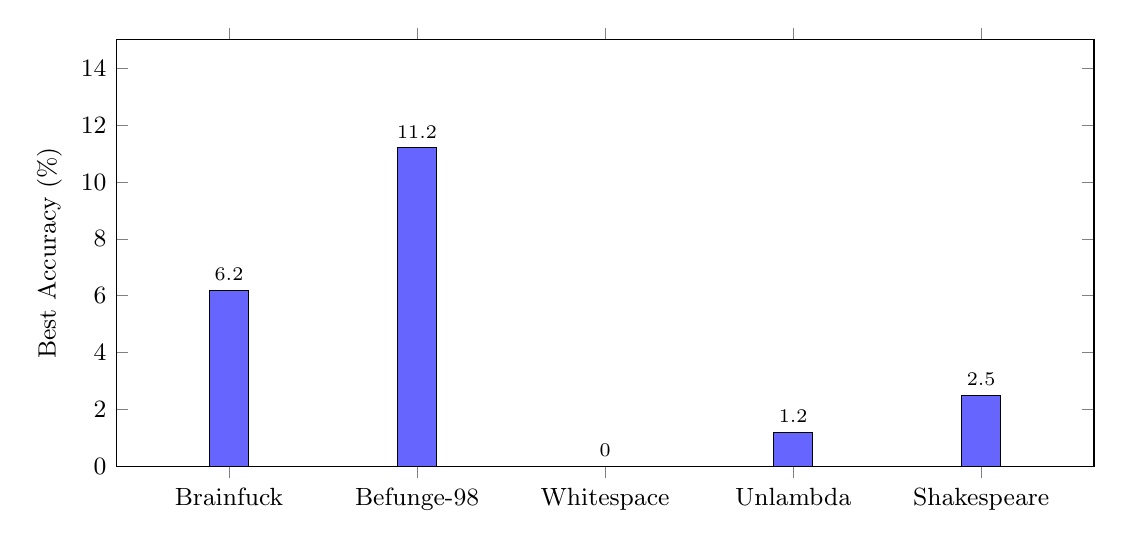
\begin{tikzpicture}
\begin{axis}[
    ybar,
    bar width=0.5cm,
    width=14cm,
    height=7cm,
    ylabel={Best Accuracy (\%)},
    ylabel style={font=\small},
    symbolic x coords={Brainfuck, Befunge-98, Whitespace, Unlambda, Shakespeare},
    xtick=data,
    x tick label style={font=\small},
    ymin=0, ymax=15,
    ytick={0,2,4,6,8,10,12,14},
    y tick label style={font=\small},
    nodes near coords,
    nodes near coords style={font=\scriptsize},
    enlarge x limits=0.15,
]
\addplot[fill=blue!60] coordinates {(Brainfuck,6.2) (Befunge-98,11.2) (Whitespace,0) (Unlambda,1.2) (Shakespeare,2.5)};
\end{axis}
\end{tikzpicture}
\caption{Best accuracy achieved per language (across all models and strategies). Befunge-98 is the most tractable (11.2\%), while Whitespace remains completely unsolved (0\%).}
\label{fig:app-lang-perf}
\end{figure}

\begin{figure}[h]
\centering
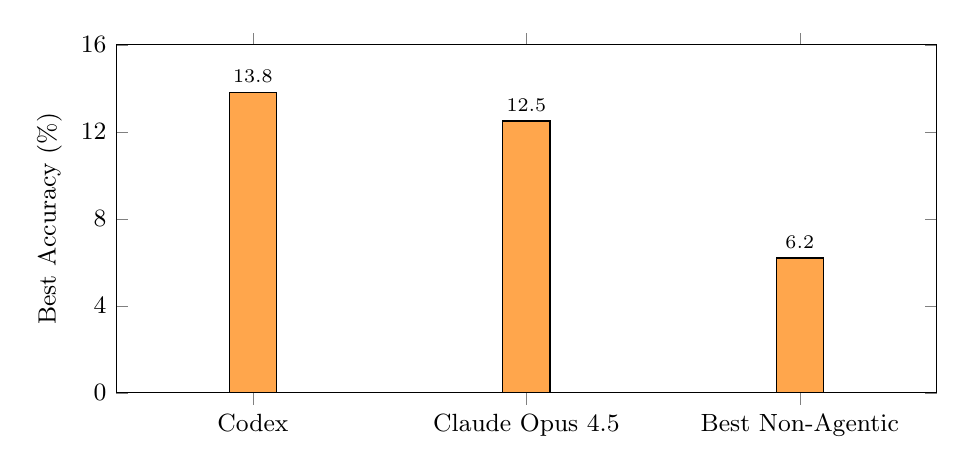
\begin{tikzpicture}
\begin{axis}[
    ybar,
    bar width=0.6cm,
    width=12cm,
    height=6cm,
    ylabel={Best Accuracy (\%)},
    ylabel style={font=\small},
    symbolic x coords={Codex, Claude Opus 4.5, Best Non-Agentic},
    xtick=data,
    x tick label style={font=\small},
    ymin=0, ymax=16,
    ytick={0,4,8,12,16},
    y tick label style={font=\small},
    nodes near coords,
    nodes near coords style={font=\scriptsize},
    enlarge x limits=0.25,
]
\addplot[fill=orange!70] coordinates {(Codex,13.8) (Claude Opus 4.5,12.5) (Best Non-Agentic,6.2)};
\end{axis}
\end{tikzpicture}
\caption{Agentic systems vs best non-agentic approach. Agentic coding systems achieve 2$\times$ higher accuracy than the best self-scaffolding approach.}
\label{fig:app-agentic}
\end{figure}

\section{Prompting Templates}
\label{app:prompts}

This section provides the exact prompts used for each strategy. Variables in \texttt{\{braces\}} are filled at runtime.

\subsection{Zero-Shot Prompt}

\textbf{System Prompt:}
\begin{verbatim}
You are an expert {language_name} programmer. Given a
problem and sample tests, output ONLY valid code in
this esoteric language. No explanations, no comments,
no markdown. Programs must read stdin exactly as
specified and write deterministic stdout that matches
the expected output byte-for-byte.

Reference documentation:
{documentation_text}
\end{verbatim}

\textbf{User Prompt:}
\begin{verbatim}
Problem ID: {problem_id}
Title: {problem_title}
Description:
{problem_description}

Specification tests (stdin => stdout):
1.
Input:
{test_1_input}
Output:
{test_1_output}

2.
Input:
{test_2_input}
Output:
{test_2_output}

[... additional test cases ...]

Return only the program.
\end{verbatim}

\subsection{Few-Shot Prompt}

Extends zero-shot by adding to the system prompt:
\begin{verbatim}
Here are solved examples for reference.
\end{verbatim}

And prepending reference examples before the problem:
\begin{verbatim}
Example 1: {example_title}
Task: {example_description}
Program:
{example_program}
Sample I/O:
- Input: {io_1_input}
  Output: {io_1_output}

Example 2: {example_title}
[... 3 examples total ...]
\end{verbatim}

\subsection{Self-Scaffolding Prompt}

\textbf{System Prompt (extends zero-shot):}
\begin{verbatim}
[Zero-shot system prompt]
Iteratively update your program using the prior code
and interpreter feedback provided.
\end{verbatim}

\textbf{User Prompt (after first attempt):}
\begin{verbatim}
[Problem specification]

Previous attempt and interpreter feedback:
=== Program ===
{previous_code}

=== Interpreter Feedback ===
Test 1:
Input: {test_input}
Expected: {expected_output}
Actual: {actual_output}
Error Type: {error_type}
Stderr: {stderr}

[... additional test results ...]

Return only the updated program.
\end{verbatim}

\subsection{Textual Self-Scaffolding Prompt}

Uses two separate prompts for coder and critic roles.

\textbf{Coder System Prompt:}
\begin{verbatim}
[Zero-shot system prompt]
Iteratively improve your solution when feedback
is provided.
\end{verbatim}

\textbf{Coder User Prompt (with feedback):}
\begin{verbatim}
[Problem specification]

Previous attempt:
{previous_code}

Critic feedback:
{critic_feedback}

Return only the updated program.
\end{verbatim}

\textbf{Critic System Prompt:}
\begin{verbatim}
You are an expert {language_name} reviewer. Analyse
the failing program and interpreter feedback. Explain
issues and suggest improvements in natural language
only. Do not write code.
\end{verbatim}

\textbf{Critic User Prompt:}
\begin{verbatim}
Problem ID: {problem_id}
Title: {problem_title}
Description:
{problem_description}

Attempt details:
=== Program ===
{code}

=== Interpreter Feedback ===
[Test results with expected/actual outputs]

Provide concise debugging guidance without including
any code.
\end{verbatim}

\subsection{ReAct Pipeline Prompt}

\textbf{Planner Prompt:}
\begin{verbatim}
Analyze this problem and create a step-by-step
algorithm in pseudocode:

Problem: {problem_description}
Test Cases: {test_cases}

Output a clear, numbered algorithm that can be
translated to any programming language.
\end{verbatim}

\textbf{Code Editor Prompt:}
\begin{verbatim}
Translate this algorithm to {language_name}:

Algorithm:
{planner_output}

Language Documentation:
{documentation}

Output only the program, no explanations.
\end{verbatim}

\textbf{Critic Prompt:}
\begin{verbatim}
The {language_name} program produced incorrect output.

Expected: {expected_output}
Actual: {actual_output}
Error: {error_type}

Analyze the discrepancy and suggest specific changes
to the algorithm or implementation.
\end{verbatim}

\section{Interpreter Specifications}
\label{app:interpreters}

All interpreters are implemented in Python with consistent interfaces:

\begin{verbatim}
result = interpreter.run(
    code: str,
    stdin: str = None,
    timeout_seconds: float = 5.0
) -> ExecutionResult

@dataclass
class ExecutionResult:
    stdout: str           # Program output
    stderr: str           # Error messages
    exit_code: int        # 0 = success
    error_type: str       # "ok", "compile_error",
                          # "runtime_error", "timeout"
\end{verbatim}

\subsection{Supported Languages}

\begin{itemize}
    \item \textbf{Brainfuck}: 30,000-cell tape, 8-bit cells with wraparound, 8 commands
    \item \textbf{Befunge-98}: 2D grid with toroidal wrapping, 200,000 step limit
    \item \textbf{Whitespace}: Stack-based with heap, 28 instructions encoded in whitespace
    \item \textbf{Unlambda}: Functional with S, K, I combinators and character I/O
    \item \textbf{Shakespeare}: Variable-per-character model with stack operations
\end{itemize}

\section{Full Problem List}
\label{app:problems}

\subsection{Easy Problems (E01-E20)}

\begin{enumerate}
    \item[E01] Print Hello World
    \item[E02] Echo Line
    \item[E03] Hello Name
    \item[E04] Sum Two Integers
    \item[E05] Multiply Two Integers
    \item[E06] Even Or Odd
    \item[E07] String Length
    \item[E08] Reverse String
    \item[E09] Count Vowels
    \item[E10] Sum From 1 To N
    \item[E11] Sum Of Digits
    \item[E12] Minimum Of Two
    \item[E13] Maximum Of Three
    \item[E14] Repeat String N Times
    \item[E15] Concatenate Two Lines
    \item[E16] First And Last Character
    \item[E17] Uppercase String
    \item[E18] Count Spaces
    \item[E19] Integer Average Of Two
    \item[E20] Compare Two Integers
\end{enumerate}

\subsection{Medium Problems (M01-M20)}

\begin{enumerate}
    \item[M01] Palindrome Check
    \item[M02] Word Count
    \item[M03] Run Length Encoding
    \item[M04] Caesar Shift By 3
    \item[M05] Simple Binary Expression
    \item[M06] Greatest Common Divisor
    \item[M07] Factorial
    \item[M08] Nth Fibonacci Number
    \item[M09] Decimal To Binary
    \item[M10] Binary To Decimal
    \item[M11] Substring Occurrences
    \item[M12] Remove Vowels
    \item[M13] Sort Numbers
    \item[M14] Second Largest Distinct Number
    \item[M15] Anagram Test
    \item[M16] Interleave Two Strings
    \item[M17] Replace Spaces With Underscores
    \item[M18] Sum Of List
    \item[M19] Characters At Even Indices
    \item[M20] Count Distinct Characters
\end{enumerate}

\subsection{Hard Problems (H01-H20)}

\begin{enumerate}
    \item[H01] Balanced Parentheses
    \item[H02] Evaluate Expression With Precedence
    \item[H03] Count Primes Up To N
    \item[H04] Nth Prime Number
    \item[H05] Big Integer Addition
    \item[H06] Longest Word
    \item[H07] Longest Common Prefix
    \item[H08] Digit Frequency
    \item[H09] General Caesar Cipher
    \item[H10] Remove Consecutive Duplicates
    \item[H11] Run Length Decoding
    \item[H12] ASCII Sum
    \item[H13] Polynomial Evaluation
    \item[H14] List All Divisors
    \item[H15] Tape Walk Final Position
    \item[H16] Longest Run Length
    \item[H17] Most Frequent Value
    \item[H18] Divisible By 3
    \item[H19] Plus Minus Reset Machine
    \item[H20] Sort Strings Lexicographically
\end{enumerate}

\subsection{Extra-Hard Problems (X01-X20)}

\begin{enumerate}
    \item[X01] Prime Factorization
    \item[X02] Longest Increasing Subsequence Length
    \item[X03] Matrix Multiplication Result Element
    \item[X04] Evaluate Postfix Expression
    \item[X05] Merge Two Sorted Arrays
    \item[X06] Compute Power Modulo
    \item[X07] Longest Palindromic Substring Length
    \item[X08] Count Set Bits In Range
    \item[X09] Bracket Depth Maximum
    \item[X10] String Rotation Check
    \item[X11] Count Inversions
    \item[X12] Least Common Multiple
    \item[X13] Valid Parentheses Types
    \item[X14] Next Greater Element
    \item[X15] Spiral Matrix Traversal
    \item[X16] Hamming Distance
    \item[X17] Roman To Integer
    \item[X18] Integer To Roman
    \item[X19] Permutation Check
    \item[X20] Josephus Problem
\end{enumerate}

\section{Extended Error Analysis}
\label{app:error-analysis}

This section provides detailed error analysis across all evaluated models. Figure~\ref{fig:app-error-all} shows error distributions for O4-mini, Gemini 3 Pro, and Qwen3-235B under zero-shot conditions.

\begin{figure}[h]
\centering
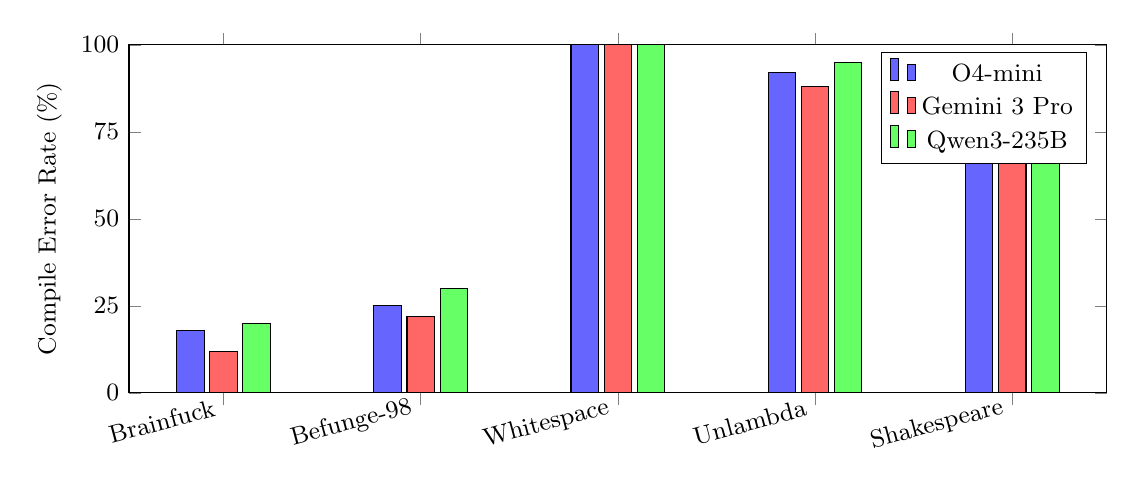
\begin{tikzpicture}
\begin{axis}[
    ybar,
    bar width=0.35cm,
    width=14cm,
    height=6cm,
    ylabel={Compile Error Rate (\%)},
    ylabel style={font=\small},
    symbolic x coords={Brainfuck, Befunge-98, Whitespace, Unlambda, Shakespeare},
    xtick=data,
    x tick label style={font=\small, rotate=15, anchor=east},
    ymin=0, ymax=100,
    ytick={0,25,50,75,100},
    y tick label style={font=\small},
    legend style={at={(0.98,0.98)}, anchor=north east, font=\small},
    enlarge x limits=0.12,
]
\addplot[fill=blue!60] coordinates {(Brainfuck,18) (Befunge-98,25) (Whitespace,100) (Unlambda,92) (Shakespeare,75)};
\addplot[fill=red!60] coordinates {(Brainfuck,12) (Befunge-98,22) (Whitespace,100) (Unlambda,88) (Shakespeare,68)};
\addplot[fill=green!60] coordinates {(Brainfuck,20) (Befunge-98,30) (Whitespace,100) (Unlambda,95) (Shakespeare,78)};
\legend{O4-mini, Gemini 3 Pro, Qwen3-235B}
\end{axis}
\end{tikzpicture}
\caption{Compile error rates by model across languages. All models show near-identical patterns: low compile errors on Brainfuck/Befunge-98, complete failure (100\%) on Whitespace, and high failure (88--95\%) on Unlambda.}
\label{fig:app-error-all}
\end{figure}

\textbf{Key observations:} (1) Error profiles are remarkably consistent across models, suggesting language-specific rather than model-specific limitations. (2) Whitespace achieves 100\% compile errors across all models---no model can generate valid whitespace-only syntax. (3) Brainfuck shows the lowest compile error rates (12--20\%) but highest logic error rates (55--65\%), indicating models can learn syntax but not semantics.

\section{Agentic System Qualitative Analysis}
\label{app:agentic-analysis}

This section provides in-depth qualitative analysis of GPT-5.2 Codex performance on Brainfuck, based on detailed execution logs from our evaluation.

\subsection{Architecture Overview}

Codex operates with an interpreter-in-the-loop architecture comprising: (1) direct interpreter access with 5 maximum attempts per problem, (2) structured logging that fetches relevant prior attempts to avoid context degradation, (3) task-family routing that retrieves semantically similar solved examples, and (4) efficient context management that mitigates the \textit{lost-in-the-middle} phenomenon by selectively surfacing relevant information rather than maintaining full conversation history.

\subsection{Performance by Problem Category}

Table~\ref{tab:codex-detailed} shows Codex performance stratified by problem category. Stream-processing problems (character I/O without numeric parsing) are solved reliably, while decimal I/O problems consistently fail.

\begin{table}[h]
\caption{Codex Brainfuck results by problem category. Stream = character-based I/O; Decimal = requires numeric parsing/printing.}
\label{tab:codex-detailed}
\begin{center}
\begin{small}
\begin{tabular}{llcc}
\toprule
\textbf{Problem} & \textbf{Category} & \textbf{Solved} & \textbf{Attempts} \\
\midrule
E01: Hello World & Stream & \checkmark & 1 \\
E02: Echo Line & Stream & \checkmark & 1 \\
E03: Hello Name & Stream & \checkmark & 1 \\
E04: Sum Two Integers & Decimal & $\times$ & 10 \\
E05: Multiply Two Integers & Decimal & $\times$ & 10 \\
E06: Even Or Odd & Classify & \checkmark & 2 \\
E07: String Length & Stream & \checkmark & 3 \\
E08: Reverse String & Stream & \checkmark & 1 \\
E09: Count Vowels & Classify & \checkmark & 3 \\
E10: Sum 1 to N & Decimal & $\times$ & 10 \\
E15: Concatenate Lines & Stream & \checkmark & 2 \\
E16: First/Last Char & Stream & \checkmark & 2 \\
E17: Uppercase String & Stream & \checkmark & 2 \\
E18: Count Spaces & Stream & \checkmark & 2 \\
\bottomrule
\end{tabular}
\end{small}
\end{center}
\end{table}

\subsection{Case Study: Successful Problem (E01)}

\textbf{Problem:} Print ``Hello World!'' with no input.

\textbf{Attempt 1 (Success):} Codex retrieves a canonical Hello World implementation from its ICL examples and generates:
\begin{verbatim}
++++++++++[>+++++++>++++++++++>+++>+<<<<-]
>++.>+.+++++++..+++.>++.<<+++++++++++++++.
>.+++.------.--------.>+.
\end{verbatim}

This solution uses standard Brainfuck idioms: initialize cells via multiplication loops, then output characters. Solved in 1 attempt with direct pattern retrieval.

\subsection{Case Study: Failed Problem (E04)}

\textbf{Problem:} Read two integers separated by whitespace, output their sum.

\textbf{Attempt 1:} Model assumes single-digit operands, produces incorrect output ``<'' for input ``5 7'' (expected ``12'').

\textbf{Attempt 2:} Attempts to split digits into cells but fails to handle multi-digit numbers.

\textbf{Attempts 3--10:} Model increasingly degenerates, trying constant outputs (``12'', ``0'', ``='') and echo strategies that cannot generalize.

\textbf{Analysis:} Decimal I/O in Brainfuck requires: (1) parsing ASCII digits into numeric values, (2) handling variable-length numbers, (3) performing arithmetic on multi-cell representations, and (4) converting results back to ASCII. This ``decimal toolkit'' pattern appears in $<$0.1\% of Brainfuck programs online, making it effectively out-of-distribution even for the highest-resource esoteric language.

\subsection{Architectural Insights}

The interpreter-in-the-loop architecture provides three key advantages for OOD tasks:

\textbf{1. Sharp feedback signal.} Direct execution output (``actual: <, expected: 12'') provides unambiguous error signal, unlike textual critique which may misdiagnose issues in unfamiliar domains.

\textbf{2. Context efficiency.} By logging attempts as structured JSON and fetching only relevant prior attempts, Codex avoids the attention dilution that occurs when LLMs must attend to long conversation histories.

\textbf{3. Task-family retrieval.} Routing problems to semantic categories (stream, classify, arithmetic) and retrieving category-specific examples outperforms generic few-shot demonstrations.

However, these advantages cannot overcome fundamental capability gaps: when the required algorithmic pattern (e.g., decimal parsing) is absent from pre-training, no amount of iteration or retrieval can synthesize it from first principles.

\end{document}
